\documentclass[11pt,a4paper,twoside,openright]{report}

\usepackage[top=25mm,bottom=25mm,right=25mm,left=30mm,head=12.5mm,foot=12.5mm]{geometry}
\let\openright=\cleardoublepage

\usepackage[a-2u]{pdfx}

\usepackage[
   backend=biber
%  ,style=iso-authoryear
  ,style=alphabetic
  ,citestyle=numeric
  ,sortlocale=cs_CZ
  ,bibencoding=UTF8
  %,block=ragged
]{biblatex}
\addbibresource{references.bib}

%% Přepneme na českou sazbu, fonty Latin Modern a kódování češtiny
\usepackage[czech]{babel}
\usepackage{lmodern}
\usepackage[T1]{fontenc}
\usepackage{textcomp}
\usepackage[utf8]{inputenc}

% Set fonts
\RequirePackage[osf]{mathpazo} % Palatino with oldstyle figures
\newcommand\liningnums[1]{\fontfamily{ppl}\selectfont#1}
\RequirePackage{eulervm}
\RequirePackage[scaled=.8819]{sourcecodepro} % Source Code Pro typeface for monospace

%%% Další užitečné balíčky (jsou součástí běžných distribucí LaTeXu)
\usepackage{amsmath}        % rozšíření pro sazbu matematiky
\usepackage{amsfonts}       % matematické fonty
\usepackage{amsthm}         % sazba vět, definic apod.
\usepackage{bm}             % tučné symboly (příkaz \bm)
\usepackage{graphicx}       % vkládání obrázků
\usepackage{fancyvrb}       % vylepšené prostředí pro strojové písmo
\usepackage{fancyhdr}       % prostředí pohodlnější nastavení hlavy a paty stránek
\usepackage{icomma}         % inteligetní čárka v matematickém módu
\usepackage{dcolumn}        % lepší zarovnání sloupců v tabulkách
\usepackage{booktabs}       % lepší vodorovné linky v tabulkách
\makeatletter
\@ifpackageloaded{xcolor}{
   \@ifpackagewith{xcolor}{usenames}{}{\PassOptionsToPackage{usenames}{xcolor}}
  }{\usepackage[usenames]{xcolor}} % barevná sazba
\makeatother
\usepackage{multicol}       % práce s více sloupci na stránce
\usepackage{caption}
\usepackage{enumitem}
\usepackage{lipsum}
\setlist[itemize]{noitemsep, topsep=0pt, partopsep=0pt}
\setlist[enumerate]{noitemsep, topsep=0pt, partopsep=0pt}
\setlist[description]{noitemsep, topsep=0pt, partopsep=0pt}
\usepackage{pdfpages}

\usepackage{tocloft}
\setlength\cftparskip{0pt}
\setlength\cftbeforechapskip{1.5ex}
\setlength\cftfigindent{0pt}
\setlength\cfttabindent{0pt}
\setlength\cftbeforeloftitleskip{0pt}
\setlength\cftbeforelottitleskip{0pt}
\setlength\cftbeforetoctitleskip{0pt}
\renewcommand{\cftlottitlefont}{\Huge\bfseries}
\renewcommand{\cftloftitlefont}{\Huge\bfseries}
\renewcommand{\cfttoctitlefont}{\Huge\bfseries}

% vyznaceni odstavcu
\parindent=0pt
\parskip=11pt

% zakaz vdov a sirotku - jednoradkovych pocatku ci koncu odstavcu na prechodu mezi strankami
\clubpenalty=1000
\widowpenalty=1000
\displaywidowpenalty=1000

% nastaveni radkovani
\renewcommand{\baselinestretch}{1.20}

% nastavení hlavy a paty stránek
\fancyhf{}
\renewcommand{\chaptermark}[1]{\markboth{#1}{}}
\fancyhead[RO,LE]{\leftmark}
\fancyfoot[RO,LE]{\thepage}
%\renewcommand{\footrulewidth}{0pt}
\fancypagestyle{plain}{%
\fancyhf{} % clear all header and footer fields
\fancyfoot[RO,LE]{\thepage}
\renewcommand{\headrulewidth}{0pt}
%\renewcommand{\footrulewidth}{0.5pt}
}

% Tato makra přesvědčují mírně ošklivým trikem LaTeX, aby hlavičky kapitol
% sázel příčetněji a nevynechával nad nimi spoustu místa. Směle ignorujte.
\makeatletter
\def\@makechapterhead#1{
  {\parindent \z@ \raggedright 
   \Huge\bfseries \thechapter. #1
   \par\nobreak
   \vskip 20\p@
}}
\def\@makeschapterhead#1{
  {\parindent \z@ \raggedright 
   \Huge\bfseries #1
   \par\nobreak
   \vskip 20\p@
}}
\makeatother

% Trochu volnější nastavení dělení slov, než je default.
\lefthyphenmin=2
\righthyphenmin=2

% Zapne černé "slimáky" na koncích řádků, které přetekly, abychom si
% jich lépe všimli.
\overfullrule=1mm

%% Balíček hyperref, kterým jdou vyrábět klikací odkazy v PDF,
%% ale hlavně ho používáme k uložení metadat do PDF (včetně obsahu).
%% Většinu nastavítek přednastaví balíček pdfx.
\hypersetup{unicode}
\hypersetup{breaklinks=true}
\hypersetup{hidelinks}

%%% Prostředí pro sazbu kódu, případně vstupu/výstupu počítačových
%%% programů. (Vyžaduje balíček fancyvrb -- fancy verbatim.)

\DefineVerbatimEnvironment{code}{Verbatim}{fontsize=\small, frame=single}



\def\NazevPrace{Webová kalkulačka podílu jednotlivce na státním rozpočtu ČR}
\def\Trida{R8.A}
\def\AutorPrace{Tomáš Hozda}
\def\DatumOdevzdani{2023}

% Vedoucí práce: Jméno a příjmení s~tituly
\def\Vedouci{Bc. Emil Miler}

% Studijní program a obor
\def\StudijniProgram{studijní program}
\def\StudijniObor{studijní obor}

% Text čestného prohlášení
\def\Prohlaseni{Prohlašuji, že jsem svou práci vypracoval samostatně a použil jsem pouze prameny a literaturu
uvedené v~seznamu bibliografických záznamů. Nemám žádné námitky proti zpřístupňování této práce v~souladu se
zákonem č. 121/2000 Sb. o~právu autorském, o~právech souvisejících s~právem autorským a
o~změně některých zákonů (autorský zákon) ve znění pozdějších předpisů.}

% Text poděkování
\def\Podekovani{%
Rád bych poděkoval rodině, přátelům, vedoucímu práce
a bratrovi za konzultaci práce.
}

% Abstrakt česky
\def\Abstrakt{%
Cílem práce je vytvořit webovou aplikaci, která funguje jako kalkulačka podílu jednotlivce na státním rozpočtu ČR. Uživatel zadá své příjmy a výdaje (různé kategorie podle zdanění) a kalkulačka vypočítá, kolik peněz za daný rok odvedl do státní rozpočtu a jak s nimi stát naložil (za co je utratil). Aplikace spravuje databázi vybraných státních výdajů a zobrazí v přepočtu, jak se uživatel na nich podílel. Databázi výdajů stejně jako státní rozpočty a průměrné hodnoty pro dané roky je možné upravovat a přidávat skrze aplikaci. Aplikace se dokáže vypořádat i s faktem, když stát utratí více, než jsou jeho příjmy. Výsledkem tak je, že uživatel z vypočítané statistiky získá obrázek o tom, jaké množství peněz odvede státu, kolik je z nich reálného užitku a k jakému účelu.
}

% Abstrakt anglicky
\def\AbstraktEN{%
The goal of the project is to create a web application, that will serve as a calculator of an individual's participation in the state budget of Czech Republic. The user will
enter their income and expenses (different categories based on taxation), and the calculator will compute, how much of his money went into the state budget, and how the state used them (that is, what it spent the money on). The application manages a database of selected state investments, and displays, how the user participated on them. The database of expenses, just like budgets and average state levies is possible to modify, add, and delete through the web interface. The app has no issue with the possibility, that the state may spent more money, than is its income. The result is that the user gets a picture, of how much money is levied from them into the state budget, and how much of it has an actual use (and which uses those are).
}

% 3 až 5 klíčových slov
\def\KlicovaSlova{daně, web, aplikace, kalkulačka, Flask, AlpineJS, PicoCSS, Nix}
% 3 až 5 klíčových slov anglicky
\def\KlicovaSlovaEN{taxes, web, application, calculator, Flask, AlpineJS, PicoCSS, Nix}


\begin{document}

%%% Titulní strana práce a další povinné informační strany

%%% Titulní strana práce

\pagestyle{empty}
\pagenumbering{gobble}
\hypersetup{pageanchor=false}

\begin{center}
\LARGE
\textbf{GYMNASIUM JANA KEPLERA}\\
{\large Parléřova 2/118, 169 00 Praha 6}

\vspace{\stretch{3}}


\includegraphics[width=.3\textwidth]{img/logo}

\vspace{\stretch{3}}

{\Huge\bfseries\NazevPrace}

\vspace{8mm}
\mdseries{Maturitní práce}

\vspace{\stretch{8}}
\large
\begin{tabular}{rl}
Autor: & \AutorPrace \\
\noalign{\vspace{2mm}}
Třída: & \Trida\\
\noalign{\vspace{2mm}}
Školní rok: & 2020/2021\\
\noalign{\vspace{2mm}}
Předmět: & Informatika \\
\noalign{\vspace{2mm}}
Vedoucí práce: & \Vedouci \\
\end{tabular}

\vspace{20mm}
Praha, \DatumOdevzdani
\end{center}


\openright

%%% 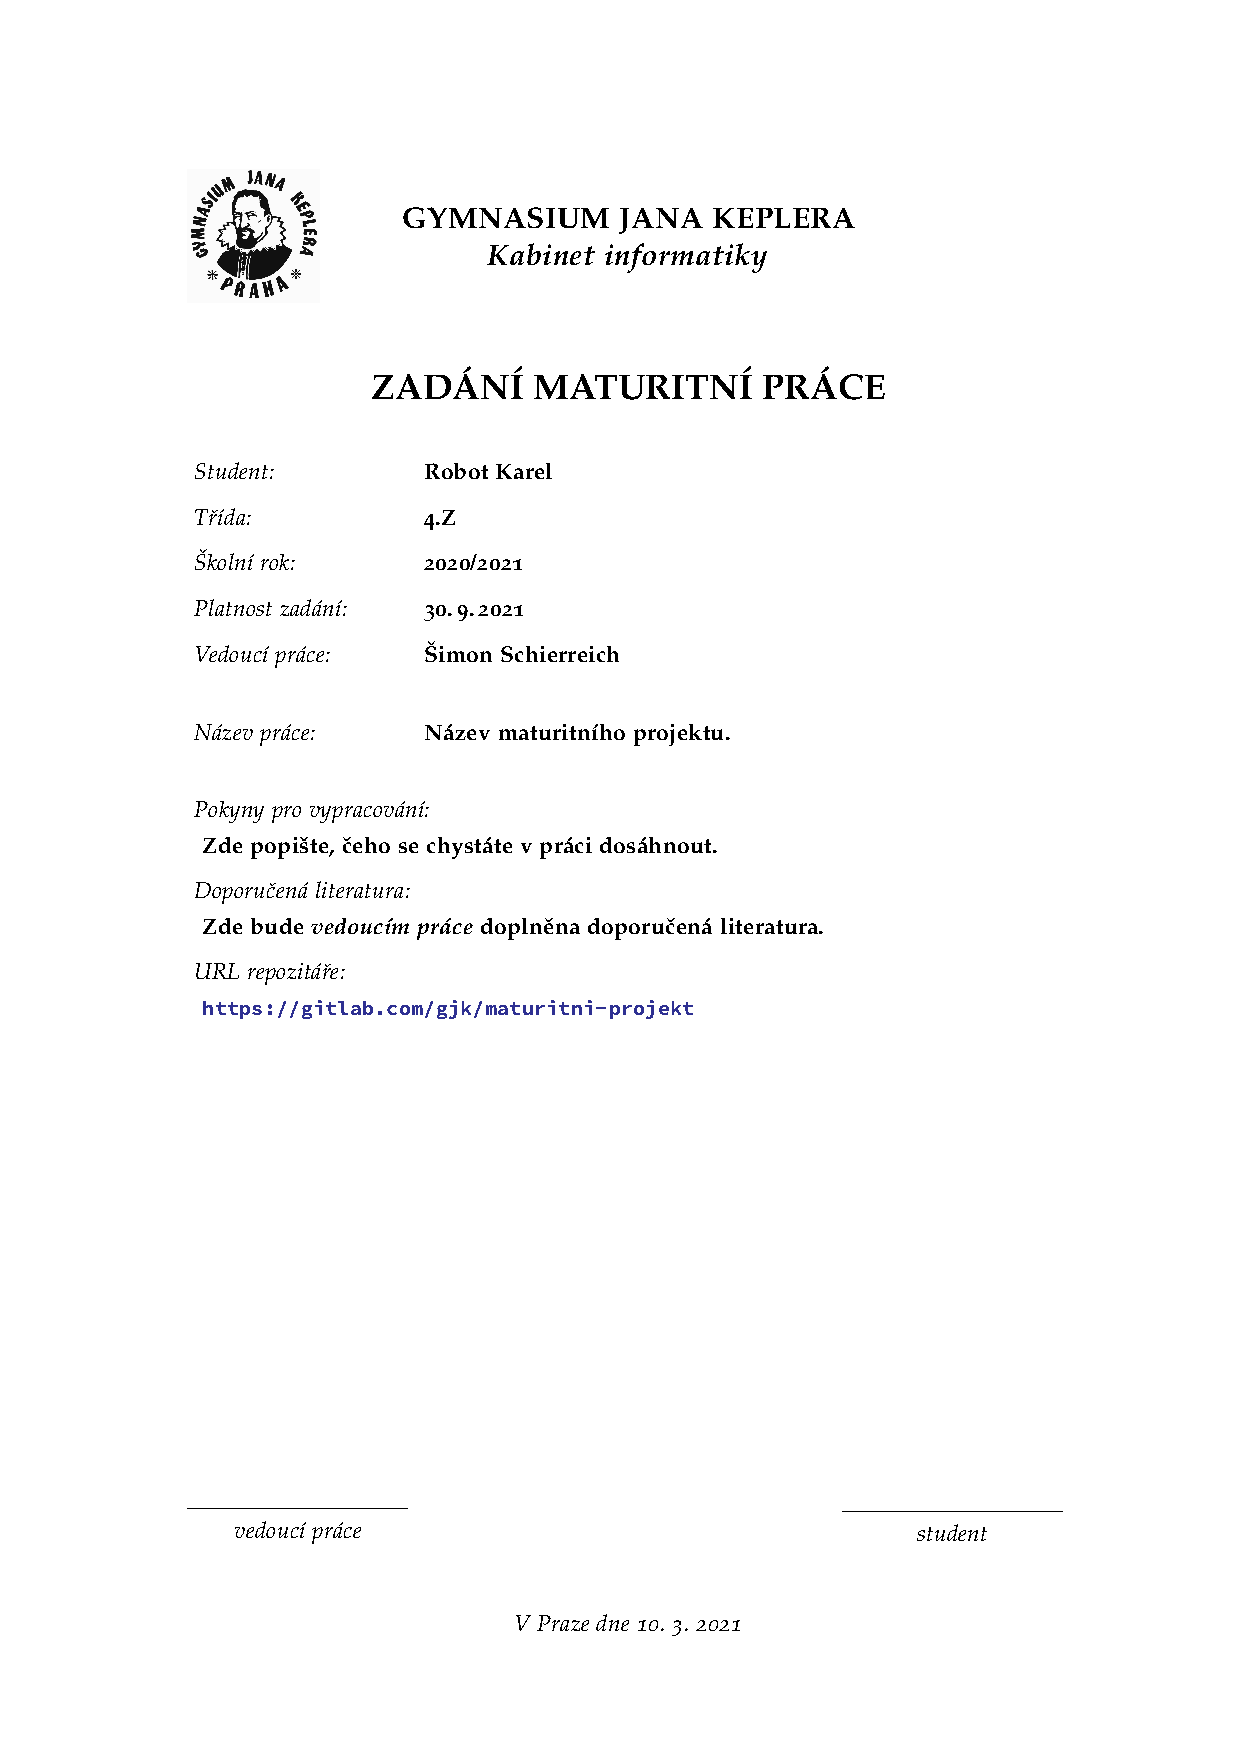
\includepdf[]{zadani.pdf}


%%% Strana s čestným prohlášením k bakalářské práci

\hypersetup{pageanchor=true}
\cleardoublepage
\vspace*{\fill}
\section*{Prohlášení}
\noindent
\Prohlaseni

\vspace{2cm}
\noindent
V Praze dne \today
\hspace*{\fill}\small{\AutorPrace}
\vspace{1cm}

%%% Poděkování
\openright
\vspace*{\fill}
\section*{Poděkování}
\noindent
\Podekovani
\vspace{1cm}


%%% Povinná informační strana bakalářské práce
\openright
\section*{Abstrakt}
\noindent
\Abstrakt
\subsection*{Klíčová slova}
\noindent
\KlicovaSlova

\vfill

\section*{Abstract}
\noindent
\AbstraktEN
\subsection*{Keywords}
\noindent
\KlicovaSlovaEN

\openright
\pagenumbering{arabic}

% Obsah
\setcounter{tocdepth}{2}
\tableofcontents

\chapter{Teoretická část}
\pagestyle{fancy}

V první části maturitní práce by se měla objevit informace o tom, jaký problém řešíte. Co si Váš projekt klade za cíl?

\section{První sekce teoretické části}

\lipsum


\chapter{Implementace}

Druhá kapitola obsahuje detailní informace o tom, jak probíhala implementace. Zde se objeví zdůvodnění výběru technologií, řešení problémů, na které jste narazili, informace o použitých knihovnách apod. Pochvalte se, nikdo to za Vás neudělá. Přiznejte chyby, není to ostuda.

\section{Ukázka sekce}

\lipsum

\chapter{Technická dokumentace}

\section{Požadavky}
Projekt je možné zprovoznit dvěma způsoby, za použití Nixu a bez něj. Postup s použitím Nixu je jednodušší a spolehlivější,
ale je použitelný pouze na Linuxových distribucích (a případně Macu), protože pro Windows nemá Nix podporu.

S Nixem jsou závislosti pro spuštění následující:

\begin{itemize}
\item Rozumná Linuxová distribuce (nebo MacOS)
\item \href{https://nixos.org/}{Nix}
\end{itemize}

V případě postupu bez Nixu je možné použít i Windows, ale je zapotřebí explicitně nainstalovat více závislostí:

\begin{itemize}
\item Python 3 (projekt byl vyvíjen s Pythonem 3.10.9, ale neměly by být problémy s kompatibilitou s novějšími verzemi)
\item PocketBase
\item \href{https://flask.palletsprojects.com/en/2.2.x/}{Flask}
\item \href{https://pypi.org/project/waitress/}{waitress} (na deployment)
\end{itemize}

Následující instrukce jsou pro Linuxové operační systémy, jakožto pro platformu, která se nejvíc hodí
na vývoj a provoz aplikací.

\subsection{Nix}
Nix je možné nainstalovat pomocí balíčkovače na vaší distribuci, například:

\begin{verbatim}
# debianovité
sudo apt-get install nix

# archovité
sudo pacman -S nix

# void linux
sudo xbps-install -Sy nix
\end{verbatim}

Doporučený je ale způsob z webové stránky Nixu\footnote{\url{https://nixos.org}}, který nainstaluje
Nix přes Nix:

\begin{verbatim}

\end{verbatim}

\subsection{Python}

\subsection{PocketBase}

\subsection{Flask}

\subsection{waitress}

\section{Instalace a spouštění}
\section{Uživatelská dokumentace}
Poslední kapitola obsahuje informace o tom, jak projekt, který v rámci maturitní práce vznikl, nainstalovat, spustit a používat.

\section{Ukázka sekce}


\subsection{A jedné podsekce}

\lipsum

\section{A další sekce}

\lipsum

\chapter*{Závěr}
\pagestyle{empty}
\addcontentsline{toc}{chapter}{Závěr}

Závěr obsahuje shrnutí práce a vyjadřuje se k míře splnění jejího zadání. Dále by se zde mělo objevit sebehodnocení studenta a informace o tom, co nového se naučil a jak vnímal svou práci na projektu.

%%% Seznam použité literatury
\nocite{einstein}\nocite{latexcompanion}\nocite{knuthwebsite}
\printbibliography[title={Seznam použité literatury},heading={bibintoc}]

%%% Seznam obrázků
\openright
\listoffigures
\addcontentsline{toc}{chapter}{Seznam obrázků}

%%% Seznam tabulek
\clearpage
\listoftables
\addcontentsline{toc}{chapter}{Seznam tabulek}

%%% Přílohy k práci, existují-li. Každá příloha musí být alespoň jednou
%%% odkazována z vlastního textu práce. Přílohy se číslují.

%\part*{Přílohy}
%\appendix

\end{document}
